% Author: Izaak Neutelings (October 2020)
\documentclass[border=3pt,tikz]{standalone}
\usepackage{physics}
\usepackage{tikz}
\usetikzlibrary{calc}
\usetikzlibrary{angles,quotes} % for pic
\usetikzlibrary{bending} % for arrow head angle
\tikzset{>=latex} % for LaTeX arrow head

\colorlet{xcol}{blue!70!black}
\colorlet{vcol}{green!60!black}
\colorlet{pcol}{red!60!black}
\colorlet{Lcol}{green!50!black}
\colorlet{myred}{red!65!black}
\colorlet{mypurple}{blue!60!red!80}
\colorlet{acol}{red!50!blue!80!black!80}
\tikzstyle{rvec}=[->,xcol,very thick,line cap=round]
\tikzstyle{vvec}=[->,vcol,very thick,line cap=round]
\tikzstyle{pvec}=[->,pcol,very thick,line cap=round]
\tikzstyle{Lvec}=[->,Lcol,very thick,line cap=round]
\tikzstyle{mass}=[line width=0.6,red!30!black,draw=red!30!black, %rounded corners=1,
                  top color=red!40!black!30,bottom color=red!40!black!10,shading angle=30]

\begin{document}


% ANGULAR MOMENTUM
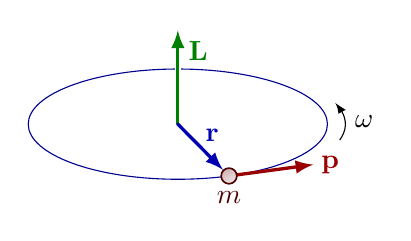
\begin{tikzpicture}
  \def\R{1.9}   % circle radius
  \def\Ry{0.7}  % circle radius
  \def\r{1.4}   % mass radius (inner sep)
  \def\ang{-70} % mass angular position
  \coordinate (O) at (0,0);
  \coordinate (L) at (0,1.7*\Ry);
  \coordinate (R) at (\ang:{\R} and \Ry);
  \draw[xcol!80!black] (O) ellipse({\R} and \Ry);
  \draw[pvec] (R) --++ (\ang+90:{0.6*\R} and 0.6*\Ry) node[right=-1] {$\vb{p}$};
  \node[mass,circle,inner sep=2] (R') at (R) {};
  \node[red!30!black,below=2] at (R') {$m$};
  \draw[white,line width=2] (O) -- (L);
  \draw[Lvec] (O) -- (L) node[below right=0] {$\vb{L}$};
  \draw[rvec] (O) -- (R') node[midway,above right=-2] {$\vb{r}$};
  \draw[-{>[bend]}] (-15:{1.12*\R} and {1.12*\Ry}) arc(-15:20:{1.12*\R} and {1.12*\Ry})
    node[pos=0.5,right] {$\omega$};
\end{tikzpicture}


% ANGULAR MOMENTUM - straight line
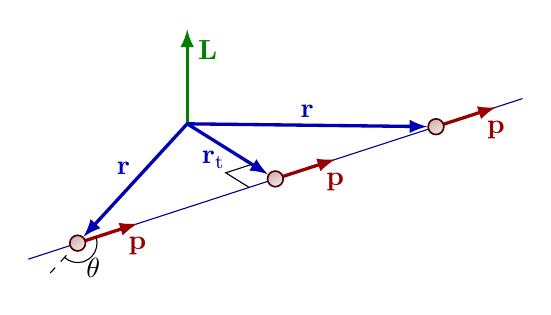
\begin{tikzpicture}
  \def\R{3.3}   % circle radius
  \def\r{1.4}   % mass radius (inner sep)
  \def\L{1.2}   % angular momentum
  \def\v{0.8}   % velocity
  \def\l{0.35}  % angular momentum
  \def\ang{18}  % mass angular position
  \def\angp{40} % angle to feign perspective
  \coordinate (O) at (\ang+90+\angp:0.4*\R);
  \coordinate (R1) at (\ang-180:0.8*\R);
  \coordinate (R2) at (0,0);
  \coordinate (R3) at (\ang:0.65*\R);
  \coordinate (R1E) at ($(O)!1.25!(R1)$); % R1 extended
  \draw[Lvec] (O) --++ (0,\L) node[below right=0] {$\vb{L}$};
  \draw[xcol!80!black] (\ang-180:\R) -- (\ang:\R);
  \draw[dashed] (R1) -- (R1E);
  \draw[pvec] (R1) --++ (\ang:\v) node[below=1] {$\vb{p}$};
  \draw[pvec] (R2) --++ (\ang:\v) node[below=1] {$\vb{p}$};
  \draw[pvec] (R3) --++ (\ang:\v) node[below=1] {$\vb{p}$};
  \node[mass,circle,inner sep=2] (R1') at (R1) {};
  \node[mass,circle,inner sep=2] (R2') at (R2) {};
  \node[mass,circle,inner sep=2] (R3') at (R3) {};
  \draw[rvec] (O) -- (R1') node[midway,above left=-2] {$\vb{r}$};
  \draw[rvec] (O) -- (R2') node[midway,below left=-3] {$\vb{r}_\mathrm{t}$};
  \draw[rvec] (O) -- (R3') node[midway,above=-1] {$\vb{r}$};
  \draw (R2)++(\ang-180:\l) --++ (\ang+90+\angp:\l) --++ (\ang:\l);
  %\draw pic["$\theta$",draw,angle radius=24,angle eccentricity=1.24] {angle=R2--R1--O};
  \draw pic["$\theta$",draw,angle radius=7,angle eccentricity=1.5] {angle=R1E--R1--R2};
\end{tikzpicture}



\end{document}
